
\section{Related \lsystem generators}

In this section a list is given of other computer programs or web pages that allow the processing of \lsystems and eventually their interpretation them in most cases as an image.

\subsection{Web based generators}
\label{sec:WebBasedGenerators}

\subsubsection{\lsystem generator by Michael Norris}
\srcurl{http://www.michaelnorris.info/software/l-system-generator.html}

\noindent
A simple script which allows one to set some basic properties of an \lsystem: namely, number of iterations, axiom and up to 15 rewrite rules.
The result is a list of strings of symbols from all iterations (it does not interpret symbols).

This site can be used to familiarize oneself with the rewriting principles of \lsystems but it offers no additional functionality.


\subsubsection{Lindenmayer power by MadFlame Software}
\srcurl{http://madflame991.blogspot.com/p/lindenmayer-power.html}

\noindent
An \lsystem generator which allows the setting of some basic properties of an \lsystem and the interpretation of each symbol.
Symbols can be interpreted using turtle graphics or they can define or modify the value of a variable.
All iterations are listed as text and also drawn on screen.

The possibility to work with variables makes it a relatively powerful system, but it is only possible to draw with a thin black line.
Also, the syntax is not very user-friendly and the user interface is hard to use (as well as the script not being very stable).
The size of the output window is only $500 \times 500$ pixels and output cannot be saved other than using print-screen.


\subsubsection{\lsystem generator by Nolan Carroll}	
\srcurl{http://nolandc.com/sandbox/fractals/}

\noindent
\lsystem generator has a nice looking interface where it is possible to set an \lsystem's basic properties.
Interpretation of symbols is fixed.
the last iteration of an \lsystem is drawn on the screen using animation (line by line from the starting position to the end).

The interface is user-friendly but the only interpretation of a symbol by drawing is a black line.
There is no help nor examples; thus, it is hard to use for an inexperienced user.
Output is drawn on a canvas which fills the entire area of the web browser but it cannot be saved other than using print-screen.


\subsubsection{VRML \lsystem generator by Patrick Murris}
\srcurl{http://www.alpix.com/vrml/lsys.htm}
  
\noindent
An \lsystem generator which can generate a 3D VRML model.
Basic properties of the \lsystem and interpretation can be set and output can be produced into VRML 1.0, 2.0 or string.

The problem is that a VRML plugin is needed for displaying 3D models.



\subsubsection{\lsystem generator by John Snyders}
\srcurl{http://hardlikesoftware.com/projects/lsystem/lsystem.html}

\noindent
At first sight this is a sophisticated \lsystem generator which can rewrite symbols with parameters and do context-sensitive rewriting.
Results can be drawn on a page as an animation of the development and a progress bar shows its status.
The biggest drawback is that \lsystems are hard-coded in JavaScript and it is only possible to change the number of iterations.

This \lsystem generator contains many examples and output is rendered as image which can be saved, but examples are the only thing that it can produce.


\subsubsection{WWW \lsystem Explorer by Zdík Kudrle}
\srcurl{http://zdeeck.borg.cz/wlse/l-system.php}

\begin{wrapfigure}{r}{0.45\textwidth}
	\vspace{-20pt}
	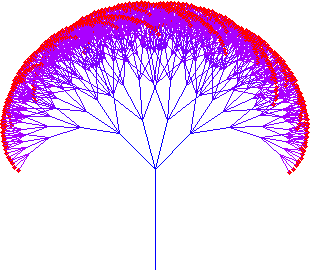
\includegraphics[width=\linewidth]{WwwLsystemExplorer}
	\caption{Image produced by WWW \lsystem Explorer}
	\label{fig:lsysExplorer}
\end{wrapfigure}

\noindent
An \lsystem generator with a well-arranged user interface where it is possible to set the basic properties of the generated \lsystems.
The interpretation of symbols is fixed and it uses an unusual set of interpretation methods like \emph{pen up} and \emph{pen down} instead of the traditional \emph{draw line} and \emph{move forward}.
The last iteration is drawn as an image by server-side PHP \nomenclature{PHP}{PHP: Hypertext preprocessor (scripting language)} script thus output can be downloaded easily.
It is possible to set line color (even to color gradient) and background color of the image.
Size of the output image can be set freely.

This web-based generator is the best among the generators listed in this section.
It contains a well-written help section and several examples.
However it cannot do context rewriting and symbols can't hold any parameters.
The length of drawn lines or turns can only be adjusted by increasing \emph{depth level} and setting the change ratio.
An example of a plant-like model produced by WWW \lsystem Explorer is shown in \autoref{fig:lsysExplorer}.



\subsection{Desktop applications}
\label{sec:DesktopGenerators}

\subsubsection{\lsystems explorer by James Matthews}
\label{sec:LsystemExplorer}
\srcurl{http://www.generation5.org/content/2002/lse.asp}

\noindent
A simple desktop application which renders \lsystems in the application window.
Basic properties of an \lsystem and its interpretation can be edited in a dialog window but interpretation of individual symbols cannot be changed.
It is possible to move and zoom the model with a mouse.
\lsystems can be saved or loaded into a text file and the drawn image can be saved to the clipboard.

\lsystems explorer can be used for generating of simple models but it is not possible to do context rewriting or use symbol parameters; even line thickness cannot be changed.
The user interface for editing an \lsystem is very simple (it is only possible to show rewrite rules for one symbol at a time).


\subsubsection{\lsystem Vector Generator by Dmitry Malutin}
\srcurl{http://xaraxtv.at.tut.by/lsvg.htm}

\begin{wrapfigure}{r}{0.4\textwidth}
	\vspace{-20pt}
	
\includegraphics[width=\linewidth]{LsystemVectorGenerator}
	\caption{A plant example from \lsystem Vector Generator}
	\label{fig:lsvg}
\end{wrapfigure}

\noindent
A similar application to \nameref{sec:LsystemExplorer} but with a better user interface and it is also possible to randomize line lengths or turn angles.
a nice feature is the \emph{angle wizard} which displays grid a of \lsystems each with a different setting of turning angle - allowing the user to easily make their choice.
Drawn lines can be automatically closed to form polygons.
It is possible to save an image as AI (Adobe Illustrator) or WMF (Windows Metafile) which are both not very common formats.

This application contains hundreds of examples but it lacks any advanced types of \lsystems or interpretation settings.
Application window size is about $700 \times 550$ pixels and it cannot be resized.
One of the built-in examples with randomized angles and line lengths is shown in \autoref{fig:lsvg}.


\subsubsection{\lsystem 4 by Timothy Perz}
\srcurl{http://www.oocities.org/tperz/L4About.htm}

\noindent
\lsystem 4 is a relatively advanced tool for generating models with \lsystems.
Besides all the basic functionality it is possible to create 3D models with custom textures.
Models can be saved as raster images (BMP or JPEG) or they can be exported to AutoCAD DXF format.
Interpreting capabilities are quite good but it can only do deterministic rewriting with a limited usage of parameters.

A table of symbol interpretations (which are not changeable) can be displayed at right-hand side of the application: a nice feature.
\lsystem 4 has good capabilities for producing 3D output but the input syntax is very compact and hard to read.
Also, more advanced \lsystem types like, context-sensitive or parametric \lsystems are, not supported.

\newcommand{\lstudio}{\mbox{L-studio}\xspace}

\subsubsection{\lstudio by Przemysław Prusinkiewicz et. al}
\srcurl{http://algorithmicbotany.org/lstudio/}

\noindent
\lstudio is probably one of the best applications designed for modeling plants with \lsystems.
\lstudio is not a single program but it is a suite of program modules that consists of many tools.
\lstudio can process all the types of \lsystems described in \autoref{sec:lsysTypes} and also produce the animation of plant growth.
With \lstudio it is possible to model 3D models of plants with regard to environmental factors such as wind, gravity, the space around a plant, sunlight, etc.
The output model can be saved in many formats such as Wavefront OBJ, Postscript, or BMP, or it can be rendered with its built-in ray-tracer to produce photo-realistic images.

There are even many examples of plant models and an extensive help section, though certainly it is not easy to start using it.
The syntax is very compact and lack clarity for a new user.

The application is not free-ware but a demo version can be downloaded.
After an evaluation period it is still possible to use it but it is not possible to export images and previews have a watermark.
In \autoref{fig:lstudio} is one of the most beautiful examples from \lstudio, the Lily.


\begin{figure}[h]
	\centering
	
\includegraphics[width=0.8\linewidth]{Lily}
	\caption{Model of Lily produced by \lstudio}
	\label{fig:lstudio}
\end{figure}





















